\documentclass[9pt,twocolumn,twoside]{gsajnl_modified}
% Use the documentclass option 'lineno' to view line numbers

\usepackage[htt]{hyphenat}  % https://tex.stackexchange.com/a/543

\PassOptionsToPackage{hyphens}{url}\usepackage{hyperref}

\articletype{inv} 

\title{Recovery of a deleted SARS-CoV-2 deep sequencing data set from the early Wuhan epidemic}

\author[]{\Large Jesse D. Bloom}

\affil[]{Fred Hutchinson Cancer Research Center}
\affil[]{Howard Hughes Medical Institute}
\affil[]{Seattle, WA, USA}

\keywords{}

\runningtitle{} % For use in the footer 
\runningauthor{}

\begin{abstract}
Abstract here
\end{abstract}

\begin{document}

\maketitle
\thispagestyle{firststyle}
%\marginmark
\firstpagefootnote

\correspondingauthoraffiliation{}{Corresponding author: \href{mailto:jbloom@fredhutch.org}{jbloom@fredhutch.org}}
\vspace{-33pt}% Only used for adjusting extra space in the left column of the first page

\lettrine[lines=2]{\color{color2}T}{}he origins... 

\section{Results}

\subsection{Identification of a SARS-CoV-2 deep sequencing data set that has been removed from the NCBI's Sequence Read Archive}
During the course of my research, I read a paper by \citet{farkas2020insights} that analyzed SARS-CoV-2 deep sequencing data from the Sequence Read Archive (SRA), which is a repository maintained by the NIH's National Center for Biotechnology Information (NCBI).
The first supplementary table of \citet{farkas2020insights} lists all SARS-CoV-2 deep sequencing data available from the SRA as of March 30, 2020.

The majority of entries in this table refer to a project (BioProject PRJNA612766) by Wuhan University that is described as nanopore sequencing of SARS-CoV-2 amplicons.
The table indicates this project represents 241 of the 282 SARS-CoV-2 sequencing run accessions in the SRA as of March, 30, 2020.
Because I had never encountered any other mention of this project, I performed a Google search for ``PRJNA612766,'' and found no search hits other than the supplementary table itself.
Searching for ``PRJNA612766'' in the NCBI's SRA search box returned a message of ``No items found.''
I then searched for individual sequencing run accessions from the project in the NCBI's SRA search box.
These searches returned messages indicating that the sequencing runs had been removed (Figure~\ref{fig:acc_removed}).

\begin{figure}[]
\centering
\fbox{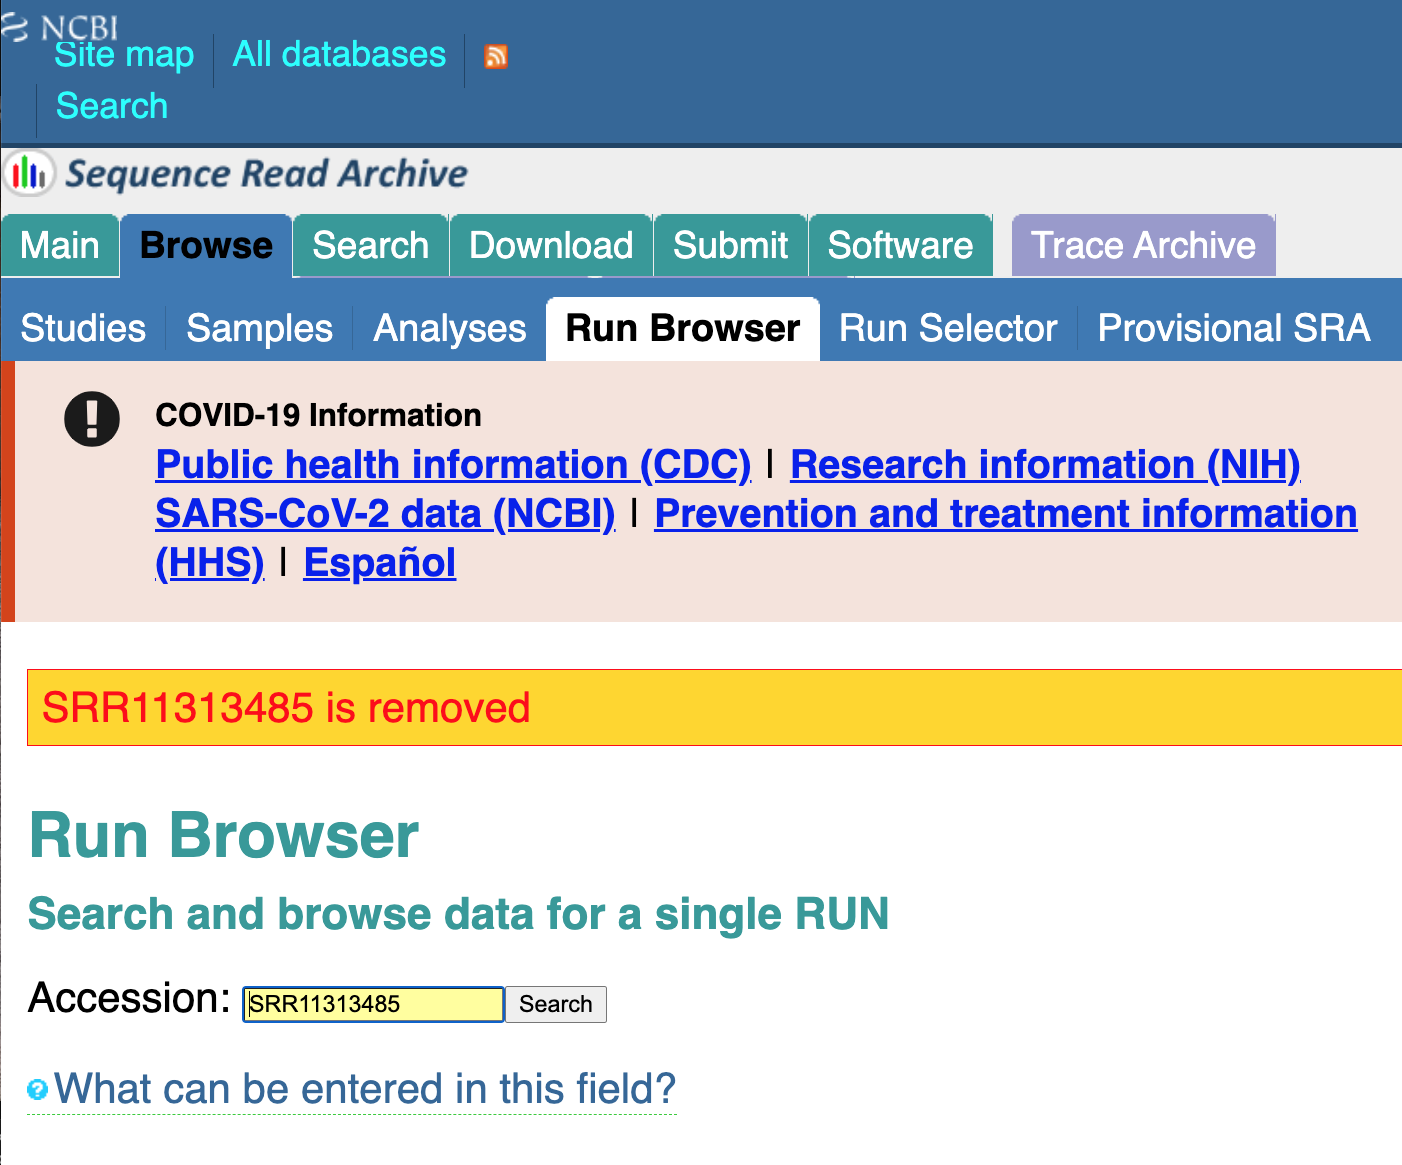
\includegraphics[trim={0.2in 0 0 9in},clip,width=\linewidth]{figures/acc_removed.png}}
\caption{Accessions from deep sequencing project PRJNA612766 have been removed from the SRA.
Shown is the result of searching for ``SRR11313485'' in the SRA search toolbar.
This result has been digitally archived on the Wayback Machine at \url{https://web.archive.org/web/20210502131630/https://trace.ncbi.nlm.nih.gov/Traces/sra/?run=SRR11313485}.
}%
\label{fig:acc_removed}
\end{figure}

The SRA is designed as a permanent archive of deep sequencing data.
The SRA documentation states that after a sequencing run is uploaded, ``neither its files can be replaced nor filenames can be changed,'' and that data can only be deleted by e-mailing SRA staff~\citep{SRA_deletion}.
An example of this process from another study is in Figure~\ref{fig:pangolin_emails}, which shows an e-mail sent to SRA staff by the lead author of a paper on pangolin coronaviruses~\citep{xiao2020isolation} to request the deletion of two sequencing runs.
Therefore, subsequent to March 30, 2020, a similar e-mail request must have been made to fully delete SARS-CoV-2 deep sequencing project PRJNA612766.

\begin{figure}[]
\centering
\fbox{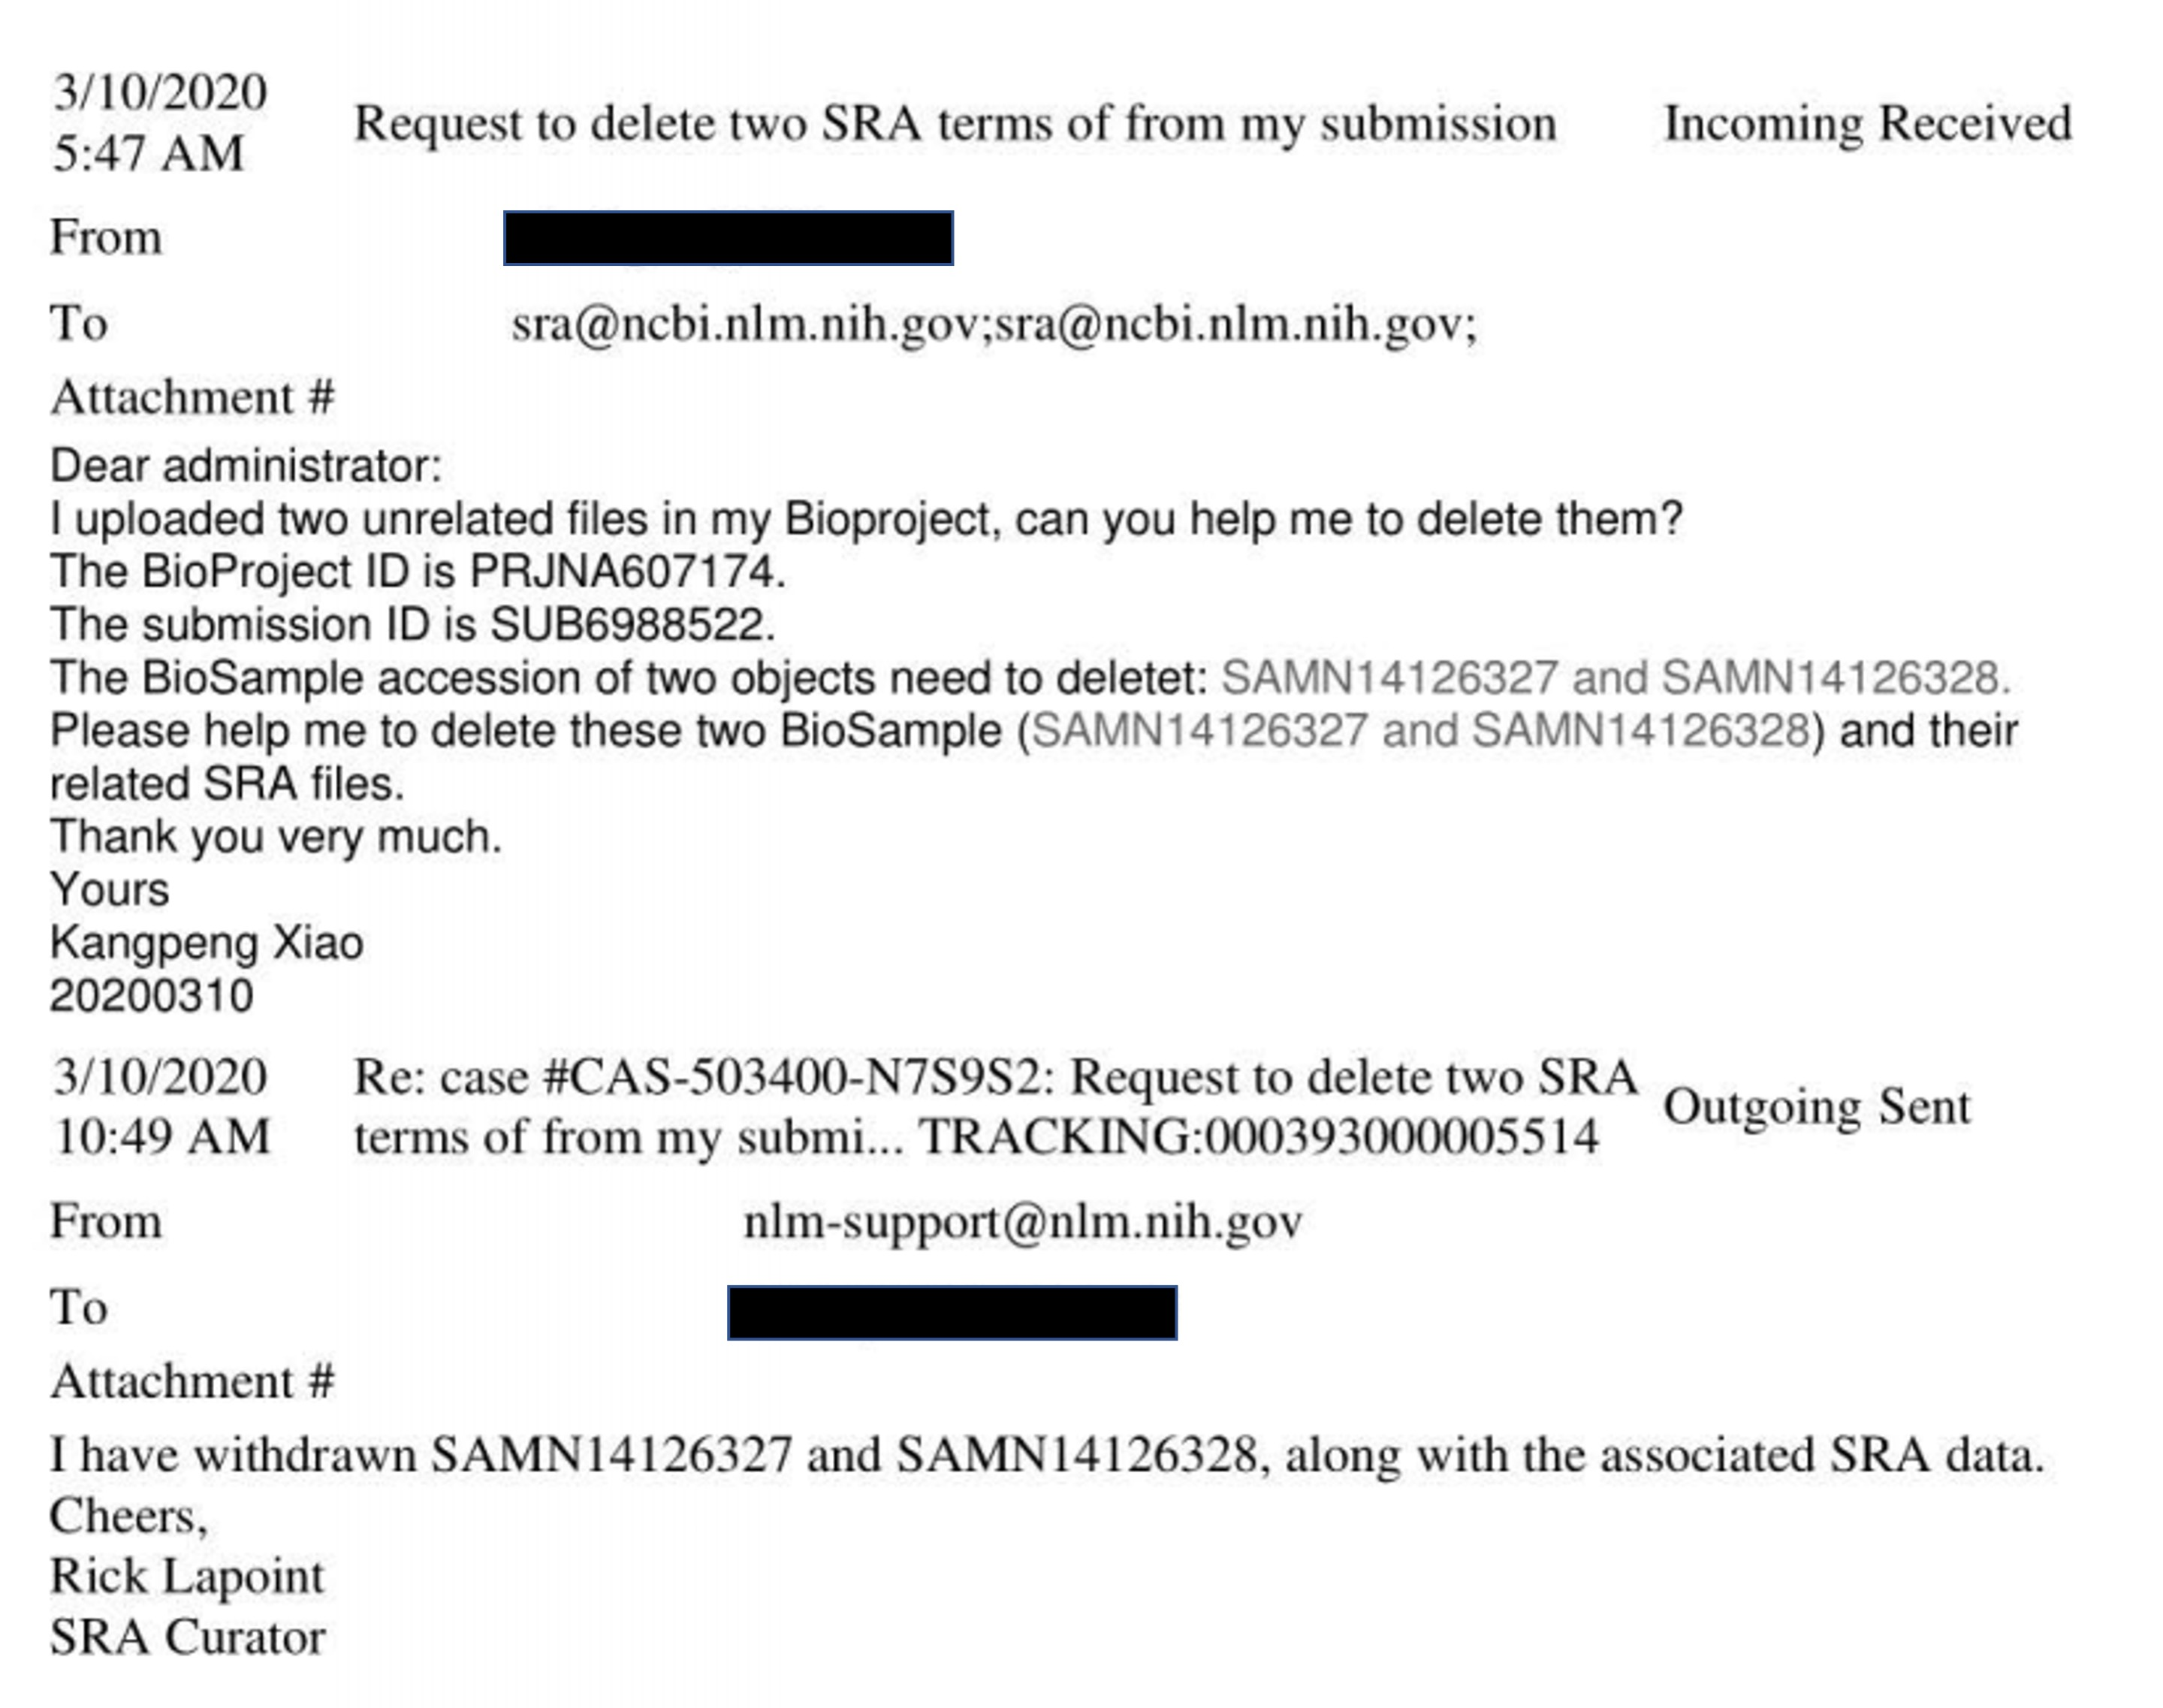
\includegraphics[trim={0.8in 0.8in 1.1in 1in},clip,width=\linewidth]{figures/pangolin_emails.jpg}}
\caption{Example of the process to delete SRA data.
The image shows excerpted e-mails between the lead author of the pangolin coronavirus paper~\citet{xiao2020isolation} and SRA staff.
The full e-mails are at \url{https://usrtk.org/tag/pangolin-papers/}.
}
\label{fig:pangolin_emails}
\end{figure}

\subsection{The deleted data set contains sequencing of viral samples collected early in the Wuhan epidemic}
The metadata in the first supplementary table of \citet{farkas2020insights} indicates that the samples in deleted project PRNJA612766 were collected by Aisu Fu and Renmin Hospital of Wuhan University.
Google searching for these terms revealed the samples were related to a study posted as a pre-print on \textit{medRxiv} in early March of 2020~\citep{wang2020medRxiv}, and subsequently published in the journal \textit{Small} in June of 2020~\citep{wang2020small}.

The study describes an approach to diagnose infection with SARS-CoV-2 and other respiratory viruses by nanopore sequencing.
This approach involved reverse-transcription of total RNA from swab samples, followed by PCR with specific primers to generate amplicons covering portions of the viral genome.
These amplicons were then sequenced on an Oxford Nanopore GridION, and infection was diagnosed if the sequencing yielded sufficient reads aligning to the viral genome.
Importantly, the study notes that this approach yields information about the sequence of the virus as well enabling diagnosis of infection.

The pre-print~\citep{wang2020medRxiv} says the approach was applied to ``45 nasopharyngeal swab samples from outpatients with suspected COVID-19 early in the epidemic.''
The digital object identifier (DOI) for the pre-print indicates that it was processed by \textit{medRxiv} on March 4, 2020, which is one day after China's State Council ordered that all papers related to COVID-19 must be approved by a centralized group to ensure that scientific publications were coordinated ``like moves in a game of chess''~\citep{Kang2020}.
The final published manuscript~\citep{wang2020small} from June of 2020 updated the description from ``early in the epidemic'' to ``early in the epidemic (January 2020).''
Both the pre-print and published manuscript say that 34 of the 45 early epidemic samples were positive in the sequencing-based diagnostic approach.
In addition, both state that the approach was later applied to 16 additional samples collected on February 11 and 12 of 2020 from SARS-CoV-2 patients hospitalized at Renmin Hospital of Wuhan University.

There is complete concordance between the accessions for project PRJNA612766 in the supplementary table of \citet{farkas2020insights} and the samples described by \citet{wang2020medRxiv}.
There are 89 accessions corresponding to the 45 early epidemic samples, with these samples named like wells in a 96-well plate (A1, A2, etc).
The number of accessions is approximately twice the number of early epidemic samples because each sample has data for two sequencing runtimes except one sample (B5) with just one runtime.
 There are 31 accessions corresponding to the 16 samples collected in February from Renmin Hospital patients, with these samples named R01, R02, etc.
 Again, all but one sample (R04) have data for two sequencing runtimes.
 In addition, there are 7 accessions corresponding to positive and negative controls, 2 accessions corresponding to other respiratory virus samples, and 112 samples corresponding to plasmids used for benchmarking of the approach.
 Together, these samples and controls account for all 241 accessions listed for PRJNA612766 in the supplementary table of \citet{farkas2020insights}.

Neither the pre-print~\citep{wang2020medRxiv} nor published manuscript~\citep{wang2020small} contain any correction or note that indicates a scientific reason for deleting the study's sequencing data from the SRA.
I e-mailed both corresponding authors of \citet{wang2020medRxiv} to ask why they had deleted the deep sequencing data and to request details on the collection dates of the early outpatient samples, but received no reply.

\subsection{Recovery of deleted sequencing data from the Google cloud} 
As indicated in Figure~\ref{fig:acc_removed}, none of the deleted sequencing runs could be accessed through the SRA's web interface.
In addition, none of the runs could be accessed using the command-line tools of the SRA Toolkit.
For instance, as of June 3, 2020, running \texttt{fastq-dump SRR11313485} or \texttt{vdb-dump SRR11313485} returned an error message stating ``err: query unauthorized while resolving query within virtual file system module - failed to resolve accession 'SRR11313485'``.

However, the SRA has begun storing all data on the Google and Amazon clouds.
While inspecting the SRA's web interface for other sequencing accessions, I noticed that SRA files are often available from links to the cloud such as \texttt{https://storage.googleapis.com/nih-sequence-read-archive/run/<ACCESSION>/<ACCESSION>}.

Based on the hypothesis that deletion of sequencing runs by the SRA might not remove files stored on the cloud, I interpolated the cloud URLs for the deleted accessions and tested if they still yielded the SRA files.
This strategy was successful; for instance, as of June 3, 2020, going to \url{https://storage.googleapis.com/nih-sequence-read-archive/run/SRR11313485/SRR11313485} downloads the SRA file for accession SRR11313485.
I have archived this file on the Wayback Machine at \url{https://web.archive.org/web/20210502130820/https://storage.googleapis.com/nih-sequence-read-archive/run/SRR11313485/SRR11313485}.

I automated this strategy to download the SRA files for 97 of the 99 sequencing runs corresponding to the 34 SARS-CoV-2 positive early epidemic samples and the 16 hospital samples from February (files for SRR11313490 and SRR11313499 were not accessible via the cloud).
I used the SRA Toolkit to get the object timestamp (\texttt{vdb-dump -{}-obj\_timestamp}) and time (\texttt{vdb-dump -{}-info}) for each SRA file.
For all files, the object timestamp is February 15, 2020, and the time is March 16, 2020.
Although the SRA Toolkit does not clearly document these two properties, my \emph{guess} is that the object timestamp may refer to when the SRA file was created from a FASTQ file uploaded to the SRA, and the time may refer to when the accession was made public.

\subsection{The data are sufficient to determine the viral sequence from the start of spike through the end of ORF10 for some samples}
The approach described by \citet{wang2020medRxiv} involved sequencing PCR amplicons covering nucleotide sites 21,563 to 29,674 of the SARS-CoV-2 genome, which spans from the start of the spike gene to the end of ORF10.
The approach also involved sequencing a short amplicon generated by nested PCR that covered a fragment of ORF1ab spanning sites $\sim$15,080 to 15,550.
In this paper, I only analyze the region from spike through ORF10 because this is a much longer contiguous sequence and the amplicons were generated by a single rather than nested PCR, which reduces the risk of PCR artifacts.
I slightly trimmed the region of interest to sites 21,570 to 29,550 because many samples had poor coverage at the very termini of the region.

\begin{figure*}[]
\centering
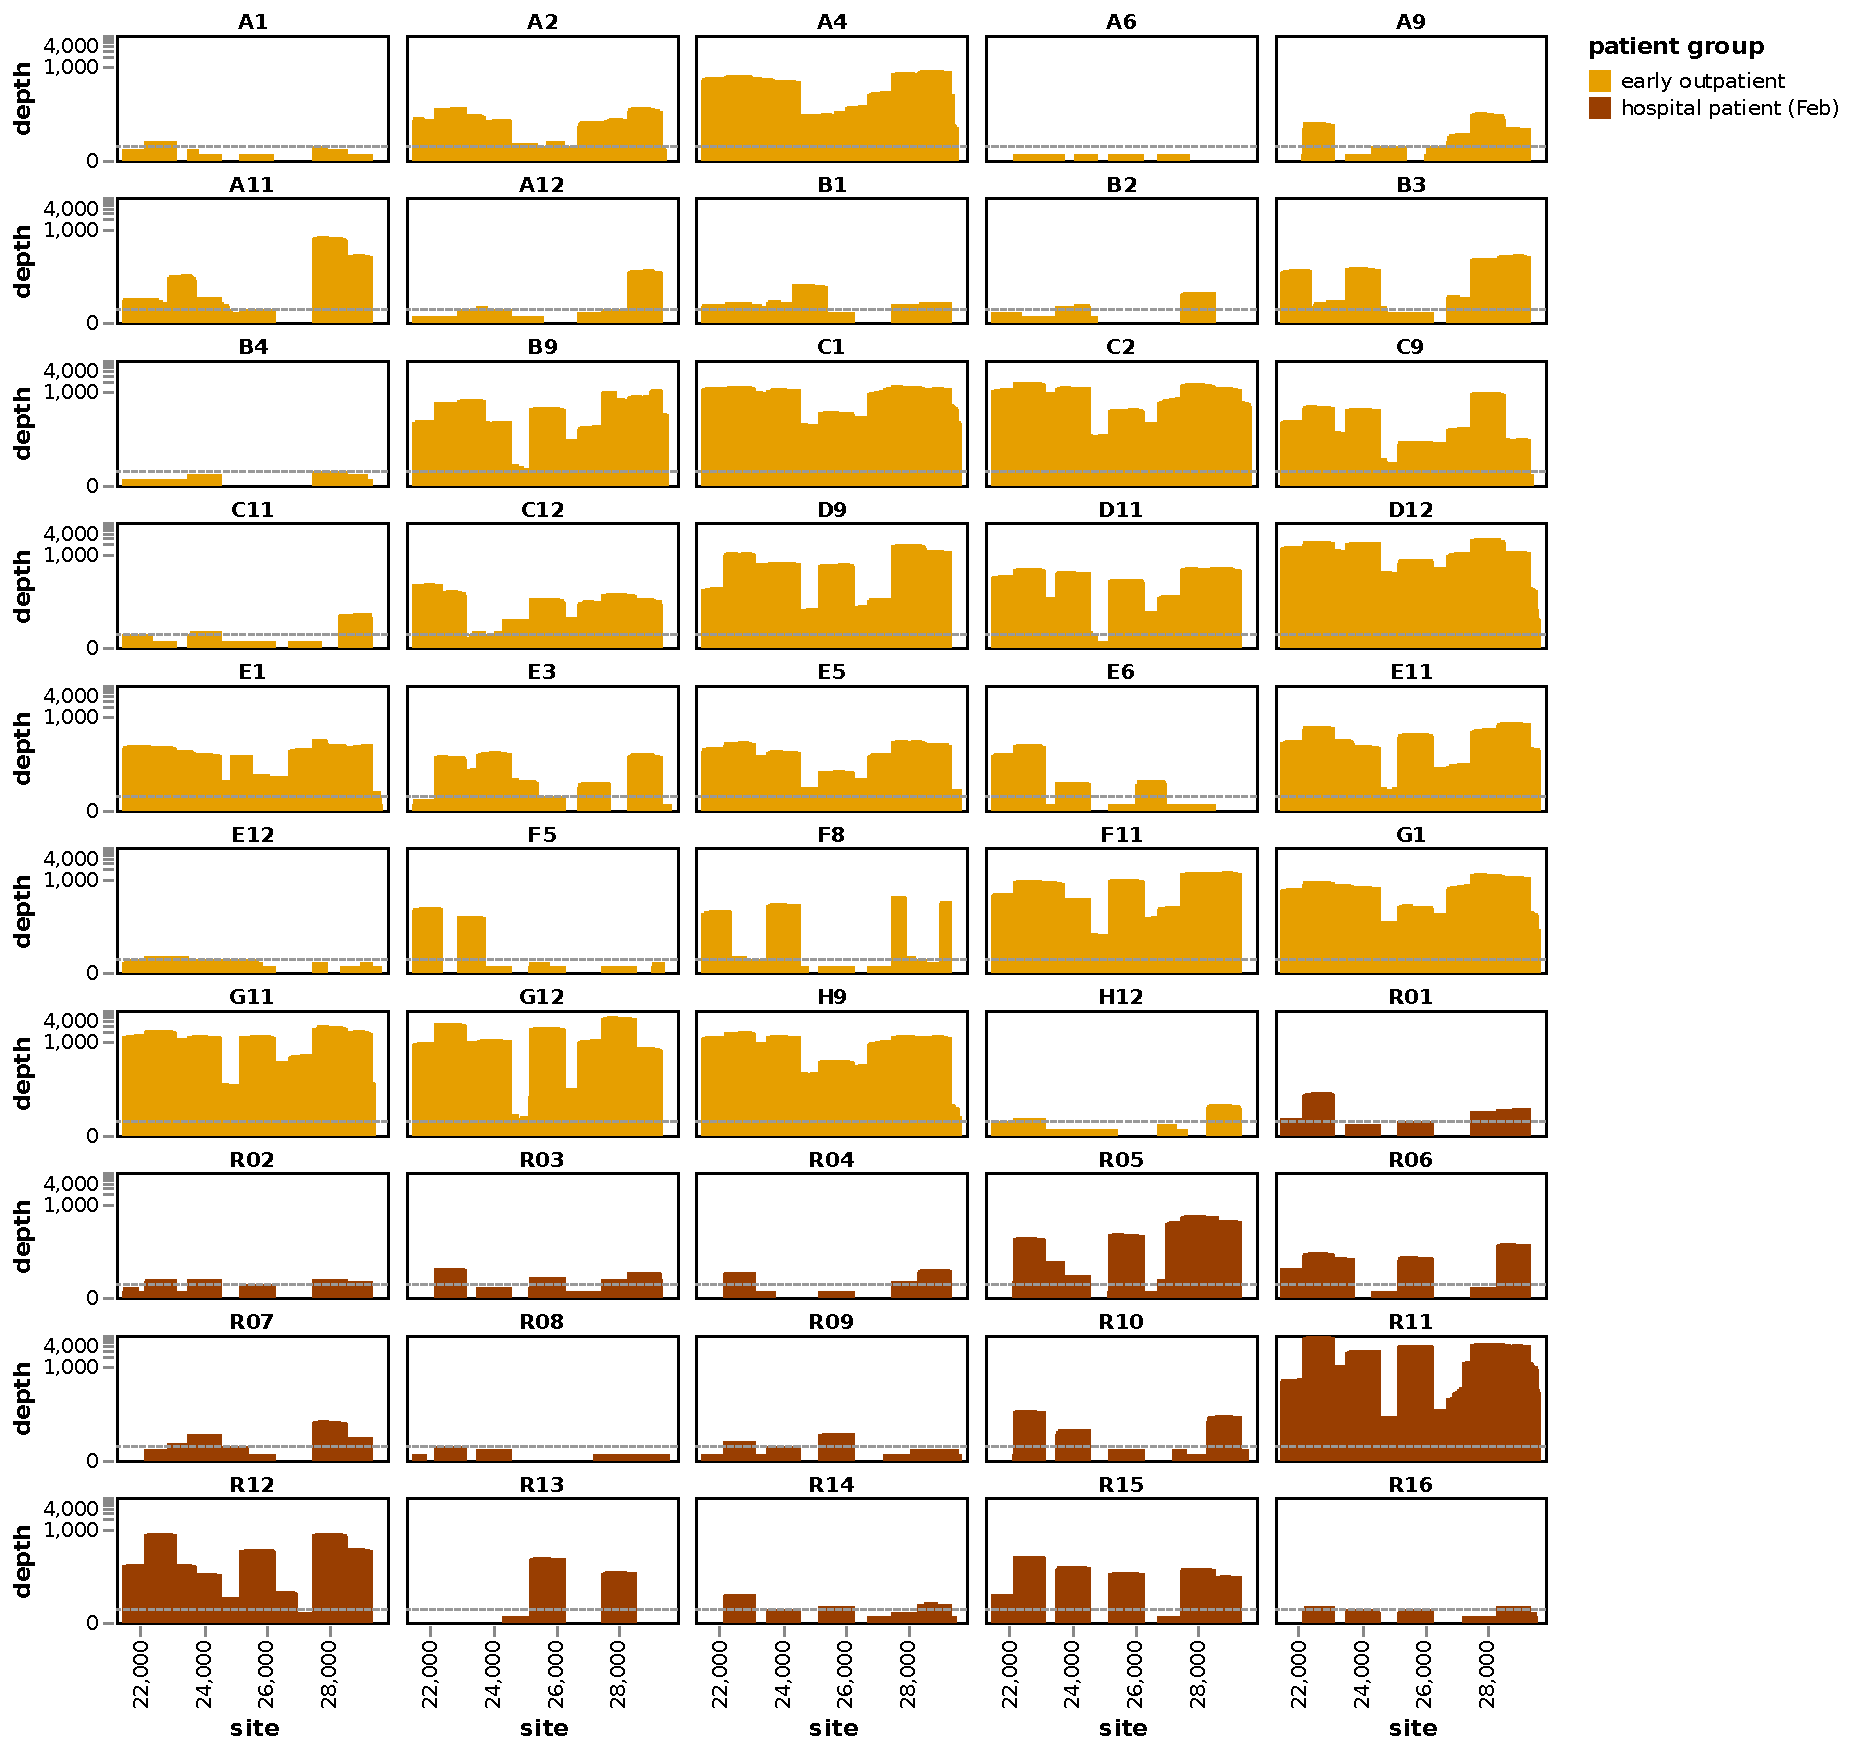
\includegraphics[width=\linewidth]{figures/coverage_region.pdf}
\caption{Sequencing depth over the SARS-CoV-2 genome from site 21,570 to 29,550 for the 34 virus-positive early outbreak samples and the 16 samples from hospitalized patients in February.
Depth is the number of aligned reads that cover that site with a quality score $\ge$20.
The dashed gray line is the minimum coverage required to call a consensus identity at a site.
Note that the y-axis uses a symlog scale.
An interactive version of this plot that enables zooming into specific site ranges and mouseovers to see read count statistics at each site is at {\color{red} add link}.
A version of the plot where the x-axis spans the entire SARS-CoV-2 genome is in Supplementary Figure~S\ref{suppfig:coverage_all}.
}
\label{fig:coverage}
\end{figure*}

I aligned the recovered deep sequencing data to the SARS-CoV-2 genome using \texttt{minimap2}~\citep{li2018minimap2}, combining accessions for the same sample.
Figure~\ref{fig:coverage} shows the sequencing coverage for the 34 virus-positive early epidemic samples and the 16 hospitalized patient samples over the region of interest; a comparable plot for the whole genome is in Supplementary Figure~S\ref{suppfig:coverage_all}.

\begin{table*}[]
{\small
\begin{tabular}{lrll}
\toprule
sample &  fraction sites called (21570-29550) &           patient group &                                        substitutions relative to proCoV2 \\
\midrule
A4 &                               0.9827 &        early outpatient &                                                                          none \\
C1 &                               0.9966 &        early outpatient &  G22081A (A=924, C=4, G=9), C28144T (C=6, T=1185), T29483G (C=1, G=45, T=1) \\
C2 &                               0.9962 &        early outpatient &                                                 C29095T (C=1, G=1, T=751)  \\
C9 &                               0.9536 &        early outpatient &                                  C28144T (C=3, T=823), G28514T (G=1, T=36)  \\
D9 &                               0.9585 &        early outpatient &                                                     C28144T (C=4, T=1653)  \\
D12 &                               0.9970 &        early outpatient &                                                     C28144T (C=8, T=2400)  \\
E1 &                               0.9759 &        early outpatient &                                                           C28144T (T=125)  \\
E5 &                               0.9758 &        early outpatient &              C24034T (A=5, C=3, T=74), T26729C (C=12), G28077C (C=142, G=4)  \\
E11 &                               0.9877 &        early outpatient &                                 C25460T (C=2, T=246), C28144T (C=1, T=412)  \\
F11 &                               0.9594 &        early outpatient &                             T25304A (A=9, T=1), C28144T (C=6, G=1, T=1328)  \\
G1 &                               0.9959 &        early outpatient &                                   none                                        \\
G11 &                               0.9677 &        early outpatient &                                  none                                         \\
H9 &                               0.9941 &        early outpatient &                                                     C28144T (C=2, T=1254)  \\
R11 &                               0.9987 &  hospital patient (Feb) &                               C21707T (T=401), C28144T (A=1, C=18, T=4265)  \\
\bottomrule
\end{tabular}
}
\caption{Samples for which the SARS-CoV-2 sequence could be called at $\ge$95\% of sites between 21,570 and 29,550, and the substitutions in this region relative to the putative SARS-CoV-2 progenitor proCoV2 inferred by \citet{kumar2021evolutionary}.
Numbers in parentheses after each substitution give the deep sequencing reads with each nucleotide identity.
\label{tab:mutations}
}
\end{table*}

I called the sequence identity at each site with coverage $\ge$3 and $>$80\% of the reads concurring on the nucleotide identity.
With these criteria, 13 of the early outpatient samples and 1 of the February hospitalized patient samples had sufficient coverage to call the nucleotide sequence at $>$95\% of the sites in the region of interest (Table~\ref{tab:mutations}), and for the remainder of this paper I focus on these high-coverage samples.
Table~\ref{tab:mutations} also shows the mutations in each sample relative to proCoV2, which is a putative progenitor of SARS-CoV-2 inferred by \citet{kumar2021evolutionary} that differs from the widely using Wuhan-Hu-1 reference sequence by three mutations (C8782T, C18060T, and T28144C).
Although requiring a coverage of only $\ge$3 is relatively lenient, Table~\ref{tab:mutations} shows that all sites with mutations are supported by at least 10 reads.
In addition, the mutations called from the raw sequences in Table~\ref{tab:mutations} concord with those mentioned in \citet{wang2020small}.

\subsection{Phylogenetic analysis of existing SARS-CoV-2 sequences from January of 2020 or earlier}
To contextualize the sequences recovered from the deleted project described above, here I first analyze early SARS-CoV-2 sequences already available in the GISAID database~\citep{shu2017gisaid}.

Numerous evolutionary analyses have shown that known human SARS-CoV-2 sequences are consistent with expansion from a single progenitor sequence~\citep{kumar2021evolutionary,pekar2021timing,rambaut2020dynamic,forster2020phylogenetic,pipes2021assessing}.
However, attempts to infer the identity of the SARS-CoV-2 progenitor sequence have been confounded by a perplexing fact: the sequences of the earliest reported isolates from Wuhan are \emph{not} the sequences most similar to SARS-CoV-2's bat coronavirus relatives~\citep{pipes2021assessing}.
Although uncertainty remains about whether the proximal origin of SARS-CoV-2 was a zoonosis~\cite{CITE} or a lab accident~\cite{CITE}, all reasonable explanations agree that at a deeper level SARS-CoV-2 genome is largely derived from one or more bat coronaviruses~\cite{CITE}.
One would therefore expect that if SARS-CoV-2 is ultimately derived from a bat coronavirus
This fact is illustrated in Figure~\ref{fig:deltadist_RaTG13}.


\begin{figure*}
\centering
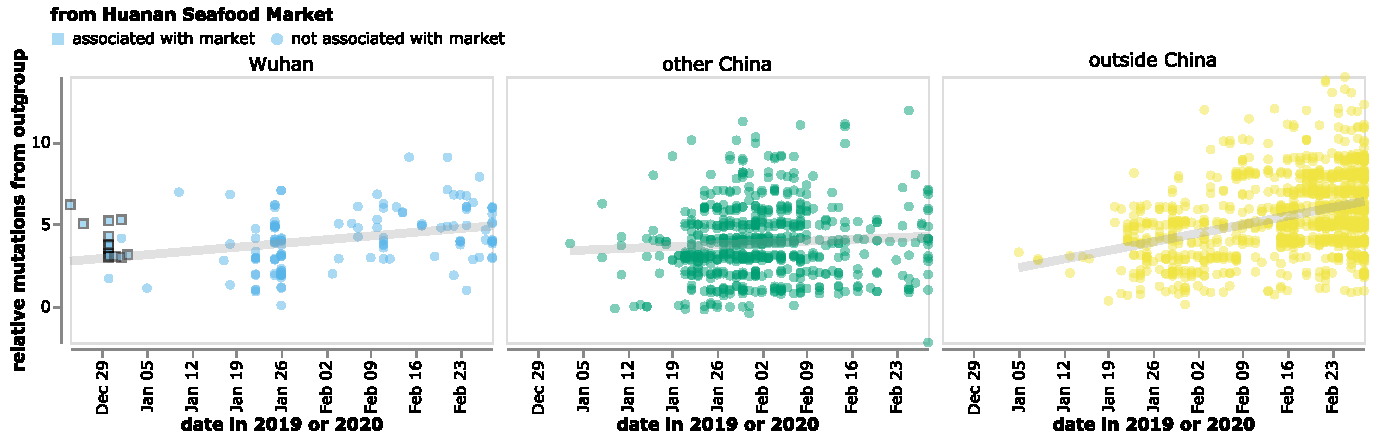
\includegraphics[width=\linewidth]{figures/deltadist_RaTG13.pdf}
\caption{The reported collection date of each SARS-CoV-2 sequence versus its relative mutational distance from the RaTG13 bat coronavirus outgroup.
Mutational distances are relative to the putative progenitor proCoV2 inferred by \citet{kumar2021evolutionary}.
The plot shows all sequences in GISAID collected no later than February 28, 2020, after performing the quality-control described in the Methods.
Sequences that the joint WHO-China report~\citep{WHO2021origins} describes as being associated with the Wuhan Seafood Market are plotted with squares.
Points are slightly jittered on the y-axis.
Go to {\color{red} add link} for an interactive version of this plot that enables toggling of the outgroup to RpYN06 and RmYN02, mouseovers to see details for each point including strain name and mutations relative to proCoV2, and adjustment of the y-axis jittering.
Static versions of the plot with RpYN06 and RmYN02 outgroups are in Supplementary Figure~\ref{suppfig:deltadist_RpYN06_RmYN02}.
}
\label{fig:deltadist_RaTG13}
\end{figure*}

\section{Methods}

\subsection{Code and data availability}
The deleted SRA files recovered from the Google cloud are all available at  \url{https://github.com/jbloom/SARS-CoV-2_PRJNA612766/tree/main/results/sra_downloads}.
I have suffixed the file extension \texttt{.sra} to all of these files.

\subsection{Archiving of key weblinks}
I have digitally archived key weblinks in the Wayback Machine.
These include:
\begin{itemize}
\item The first supplementary table of \citet{farkas2020insights}, which lists all SARS-CoV-2 accessions in the SRA as of March 30, 2020, is archived at \url{https://web.archive.org/web/20210502130356/https://dfzljdn9uc3pi.cloudfront.net/2020/9255/1/Supplementary_Table_1.xlsx}. 
\end{itemize}

\bibliography{references}

\clearpage
\onecolumn
\renewcommand{\thepage}{S\arabic{page}}
\setcounter{page}{1}

\section{Supplementary Material}

\begin{figure}[h!]
\centering
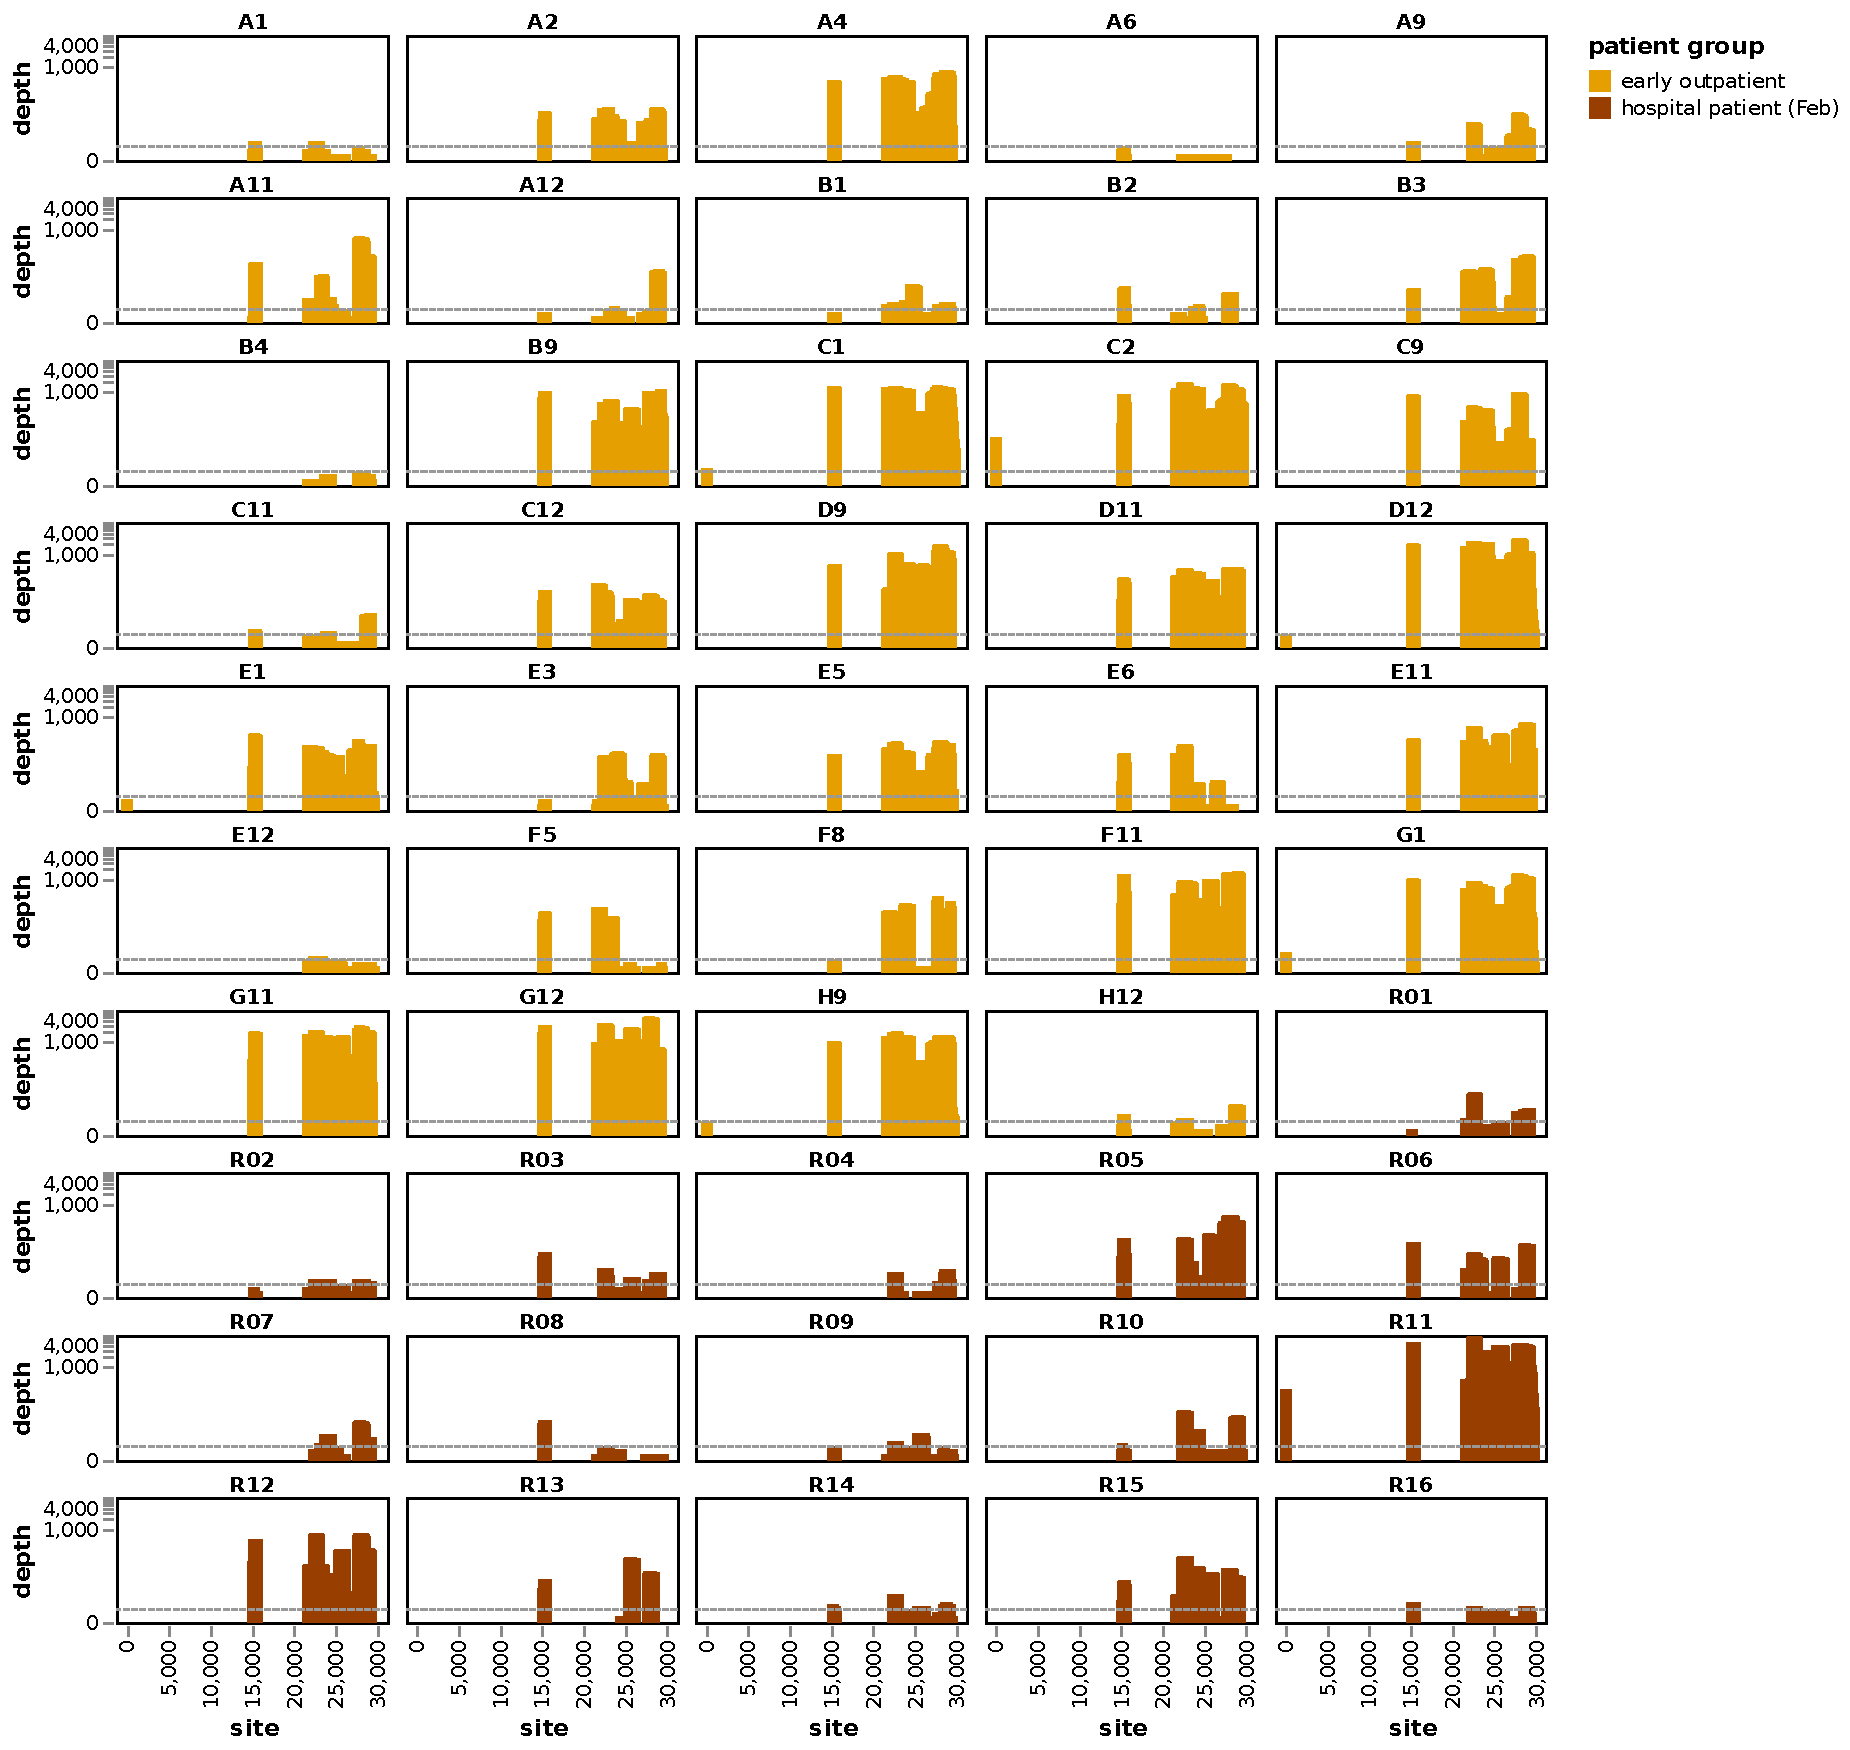
\includegraphics[width=\linewidth]{figures/coverage_all.pdf}
\caption{A version of Figure~\ref{fig:coverage} that shows coverage over the full length of the SARS-CoV-2 genome.
An interactive version of this plot is at {\color{red} add link}.
}
\label{suppfig:coverage_all}
\end{figure}

\begin{figure}[h!]
{\bf \LARGE A} \\
\centerline{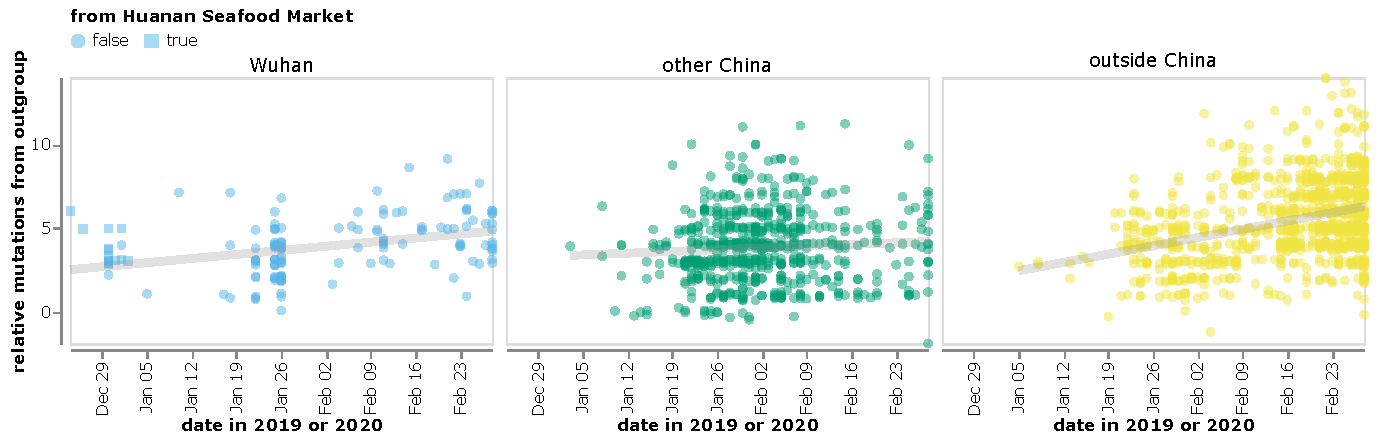
\includegraphics[width=\linewidth]{figures/deltadist_RpYN06.pdf}}
{\bf \LARGE B} \\
\centerline{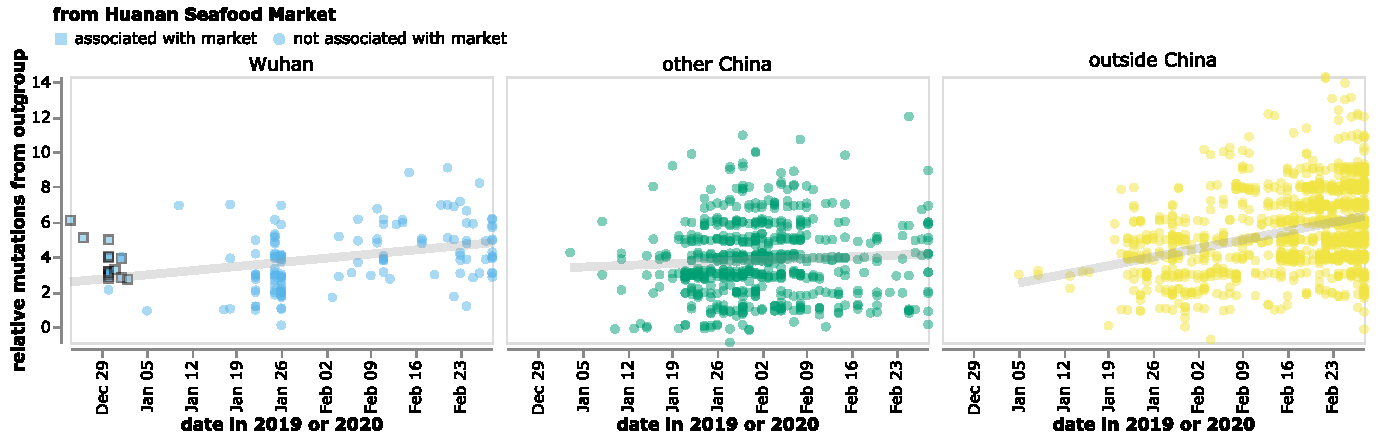
\includegraphics[width=\linewidth]{figures/deltadist_RmYN02.pdf}}
\caption{Versions of Figure~\ref{fig:deltadist_RaTG13} but calculating the relative mutational distances using an outgroup of (A) RpYN06 or (B) RmYN02.
}
\label{suppfig:deltadist_RpYN06_RmYN02}
\end{figure}



\end{document}
